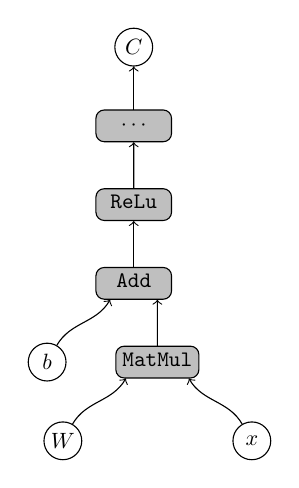
\begin{tikzpicture}
[
operator/.style = {rectangle, draw, fill = lightgray, inner sep = 3pt, font = \ttfamily\vphantom{Ag}, rounded corners = 3pt, minimum width = 1.2cm, scale = 0.8},
    tensor/.style = {circle, draw, fill = white, inner sep = 1pt, minimum size = 0.6cm, scale = 0.8}
]
    \node[tensor] (c) {$C$};
    \node[operator] (cdots) at ([yshift = -1cm]c) {$\cdots$};
    \node[operator] (relu) at ([yshift = -1cm]cdots) {ReLu};
    \node[operator] (add) at ([yshift = -1cm]relu) {Add};
    \node[operator] (matmul) at ([yshift = -1cm, xshift = 0.3cm]add) {MatMul};
    \node[tensor] (b) at ([xshift = -1.4cm]matmul) {$b$};
    \node[tensor] (w) at ([yshift = -1cm, xshift = -1.2cm]matmul) {$W$};
    \node[tensor] (x) at ([yshift = -1cm, xshift = 1.2cm]matmul) {$x$};


    \draw[->] (w) to[out = 60, in = 240] ([xshift = -0.4cm]matmul.south);
    \draw[->] (x) to[out = 120, in = -60] ([xshift = 0.4cm]matmul.south);
    \draw[->] (matmul) -- (matmul |- add.south);
    \draw[->] (b) to[out = 60, in = 240] ([xshift = -0.3cm]add.south);
    \draw[->] (add) -- (relu);
    \draw[->] (relu) -- (cdots);
    \draw[->] (cdots) -- (c);
\end{tikzpicture} 
